\documentclass[11pt]{article}


\usepackage[utf8]{inputenc}
\usepackage[T1]{fontenc}
\usepackage[french]{babel}
\usepackage{fourier}
\usepackage[scaled=0.875]{helvet}
\renewcommand{\ttdefault}{lmtt}
\usepackage{diagbox}
\usepackage{fancybox}
\usepackage[normalem]{ulem}
\usepackage{pifont}
\usepackage{lscape}
\usepackage{multicol}
\usepackage{mathrsfs}
\usepackage{tabularx,array}
\usepackage{colortbl}
\usepackage{multirow}
\usepackage{textcomp}
\usepackage{enumitem}  
\usepackage{hyperref}

% Dimensionnement fenêtre
\usepackage[left=3.5cm, right=3.5cm, top=2cm, bottom=3cm]{geometry}

%Packages utiles
%graphiques
\usepackage{fancyhdr}
\usepackage{graphicx}
\usepackage{fancybox}
\usepackage{pgf,tikz}
\usetikzlibrary{arrows}
% macro ams
\usepackage{amsfonts,amsmath,amssymb,amsthm}
%Permet de definir de nouveaux types de theoremes
\usepackage[framemethod=tikz]{mdframed}
% Pour les corrections d'exercices
\usepackage{answers}
% pour tracer des lignes (voir la commande \pointilles)
\usepackage{dashrule}
% pour répéter des commandes
\usepackage{multido}

%FONTES POUR ALGO
\DeclareFontFamily{T1}{lmtt}{} 
\DeclareFontShape{T1}{lmtt}{m}{n}{<-> ec-lmtl10}{} 
\DeclareFontShape{T1}{lmtt}{m}{\itdefault}{<-> ec-lmtlo10}{} 
\DeclareFontShape{T1}{lmtt}{\bfdefault}{n}{<-> ec-lmtk10}{} 
\DeclareFontShape{T1}{lmtt}{\bfdefault}{\itdefault}{<-> ec-lmtko10}{}
\renewcommand{\ttdefault}{lmtt}
% PACKAGES NECESSAIRES POUR ALGO
\usepackage{xcolor}
\usepackage{framed}
\usepackage[boxed]{algorithm}
\usepackage{algorithmic}
%\usepackage{algpseudocode}
%\input algolatex
\renewcommand{\algorithmicensure}{\textbf{Sortie :}}
\renewcommand{\algorithmicend}{\textbf{fin}}
\renewcommand{\algorithmicrequire}{\textbf{Variables :}}
\renewcommand{\algorithmicif}{\textbf{si}}
\renewcommand{\algorithmicthen}{\textbf{alors}}
\renewcommand{\algorithmicelse}{\textbf{sinon}}
\renewcommand{\algorithmicelsif}{\algorithmicelse\ \algorithmicif}
\renewcommand{\algorithmicendif}{\algorithmicend\ \algorithmicif}
\renewcommand{\algorithmicfor}{\textbf{pour}}
\renewcommand{\algorithmicforall}{\textbf{pour tout}}
\renewcommand{\algorithmicdo}{\textbf{faire}}
\renewcommand{\algorithmicendfor}{\algorithmicend\ \algorithmicfor}
\renewcommand{\algorithmicwhile}{\textbf{tant que}}
\renewcommand{\algorithmicendwhile}{\algorithmicend\
\algorithmicwhile}
\renewcommand{\algorithmicloop}{\textbf{boucler}}
\renewcommand{\algorithmicendloop}{\algorithmicend\
\algorithmicloop}
\renewcommand{\algorithmicrepeat}{\textbf{r\'ep\'eter}}
\renewcommand{\algorithmicuntil}{\textbf{jusqu'à }} 
\renewcommand{\algorithmicreturn}{\textbf{Afficher}} 




\title{Activité d'introduction aux algorithmes gloutons}
\author{Raphaël Bomboy\\
   Lycée Jean Perrin\\
   Lyon}
\date{\today}



%En-tetes et pieds de pages
\pagestyle{fancy}
\lhead{}
\chead{}
\rhead{}
\lfoot{}
\cfoot{}
\rfoot{\thepage}


%Definit les diff\'erents types de th\'eor\'emes et leurs styles
\theoremstyle{plain}
\newtheorem*{thme}{Theor\`eme}
\surroundwithmdframed[linecolor=black,backgroundcolor=gray!10,roundcorner=10pt]{thme}
\newtheorem*{cons}{Cons\'equence}
\surroundwithmdframed[linecolor=black,backgroundcolor=gray!10,roundcorner=10pt]{cons}
\newtheorem*{prop}{Propri\'et\'e}
\surroundwithmdframed[linecolor=black,backgroundcolor=gray!10,roundcorner=10pt]{prop}
\newtheorem*{props}{Propri\'et\'es}
\surroundwithmdframed[linecolor=black,backgroundcolor=gray!10,roundcorner=10pt]{props}
\newtheorem*{defprop}{D\'efinition-Propri\'et\'e}
\surroundwithmdframed[linecolor=black,backgroundcolor=gray!10,roundcorner=10pt]{defprop}

\theoremstyle{definition}
\newtheorem*{definition}{D\'efinition}
\surroundwithmdframed[linecolor=black,backgroundcolor=gray!10,roundcorner=10pt]{definition}
\newtheorem*{definitions}{D\'efinitions}
\surroundwithmdframed[linecolor=black,backgroundcolor=gray!10,roundcorner=10pt]{definitions}


\theoremstyle{remark}
\newtheorem*{ex}{Exemple}
%\surroundwithmdframed[linecolor=black,backgroundcolor=gray!10,roundcorner=10pt]{ex}
\newtheorem*{exs}{Exemples}
%\surroundwithmdframed[linecolor=black,backgroundcolor=gray!10,roundcorner=10pt]{exs}
\newtheorem*{att}{Attention}
%\surroundwithmdframed[linecolor=black,backgroundcolor=gray!10,roundcorner=10pt]{att}
\newtheorem*{rem}{Remarque}
%\surroundwithmdframed[linecolor=black,backgroundcolor=gray!10,roundcorner=10pt]{rem}

%D\'efinit les environnements exo et corr
\newtheoremstyle{exercice}%
{\topsep}{\topsep}%
{\normalfont}%
{}%
{\bfseries}%
{\newline}%  
{.5em}%
{}
\theoremstyle{exercice}
\newtheorem{exo}{Exercice}
\Newassociation{corr}{Soln}{mycor}
\renewcommand{\Solnlabel}[1]{Corrig\'e #1}



%Commandes utiles pour les symboles math�matiques
\newcommand{\R}{\mathbb{R}}
\newcommand{\N}{\mathbb{N}}
\newcommand{\D}{\mathbb{D}}
\newcommand{\Z}{\mathbb{Z}}
\newcommand{\Q}{\mathbb{Q}}
\newcommand{\C}{\mathbb{C}}
\newcommand{\euro}{\eurologo{}}
\newcommand{\repere}{(O,\vec{\imath},\vec{\jmath})}
\newcommand{\courbe}{\mathcal{C}}
\newcommand{\vect}[1]{ \overrightarrow{#1}}
\newcommand{\colcoord}[2]{\left(\begin{array}{c}
#1\\
#2
\end{array}\right)}
\def\e{\text{e}}
\def\i{\text{i}}
\newcommand{\ds}{\displaystyle}%   displaystyle
\newcommand{\cg}{\texttt{]}}% crochet gauche
\newcommand{\cd}{\texttt{[}}% crochet droit
\newcommand{\pg}{\geqslant}%  plus grand ou égal
\newcommand{\pp}{\leqslant}%  plus petit ou égal
\newcommand{\barre}[1]{\overline{\,\mathstrut#1\,}}
\renewcommand{\theenumi}{\textbf{\arabic{enumi}}}
\renewcommand{\labelenumi}{\textbf{\theenumi.}}
\renewcommand{\theenumii}{\textbf{\alph{enumii}}}
\renewcommand{\labelenumii}{\textbf{\theenumii.}}
\def\Oij{$\left(\text{O},~\vect{\imath},~\vect{\jmath}\right)$}
\def\Oijk{$\left(\text{O},~\vect{\imath},~\vect{\jmath},~\vect{k}\right)$}
\def\Ouv{$\left(\text{O},~\vect{u},~\vect{v}\right)$}

% pointilles
% l'argument #1 est la longueur demandée
\newlength{\textelarg}
\newcommand{\pointilles}[2]{
 \noindent {#2}%
 \settowidth{\textelarg}{#2}%
 \addtolength{\textelarg}{-.5ex}%
 \addtolength{\textelarg}{-2\textelarg}%
 \addtolength{\textelarg}{\linewidth}%
 \leavevmode\hdashrule[0ex]{\textelarg}{.005pt}{0.5mm}\kern 0pt%
 \addtolength{\textelarg}{-\textelarg} \\[0.5\parskip]%
 \multido{}{#1}{%
 \leavevmode\hdashrule[0ex]{\linewidth}{.005pt}{0.5mm}\kern 0pt\\[0.5\parskip]
 }
 \vspace*{-0.5\parskip}
}
% lpointilles
\newcommand{\lpointilles}[1]{
 \leavevmode\hdashrule[0ex]{#1}{.05pt}{1mm}\kern 0pt%
}



\begin{document}

\maketitle

\section{Objectifs et contenu de l'activité}

Nous présentons ici une activité d'introduction en enseignement à distance à la notion d’algorithme glouton, destinée à des élèves de classe de première suivant la spécialité NSI.

\medskip

 Cette introduction se fait à travers l'étude de deux problèmes classiques explicitement cités au programme : le problème du rendu de monnaie et celui du sac à dos.
 
\medskip
 
L'activité est introductive et ne se veut pas une définition complète de la notion d'algorithme glouton. Elle pourra sur le sujet être complété plus tard. De même, la terminaison et la complexité des deux algorithmes présentés ne sont pas traitées lors de cette première approche.

\section{Prérequis}

Les élèves doivent maîtriser les savoir-faire suivants~:

\begin{itemize}
	\item syntaxe de base du langage Python
	\item manipulation des listes sous Python, et de préférence des listes en compréhension
	\item utilisation élémentaire d'un Jupyter notebook.
\end{itemize}

\section{Mise en œuvre et temps imparti}

L'activité prend la forme d'un Jupyter notebook partagé en ligne au moyen de la plateforme Binder.

\medskip

Le notebook alterne :

\begin{itemize}
	\item des paragraphes de cours et de présentation des exemples
	\item des questions à résoudre à l'aide d'un papier et d'un crayon
	\item des blocs de code Python à compléter et exécuter.
\end{itemize}

\medskip

L'idée est que les élèves puissent travailler le cours en autonomie, tout en prenant le temps de répondre aux questions ainsi que de rédiger le code Python et de le tester sur différents exemples, dans l'objectif de comprendre les algorithmes décrits et de vérifier leur caractère non toujours optimal.

\medskip

L'ensemble est prévu pour environ une heure, cette durée pouvant peut-être être ambitieuse pour des élèves de première.

\section{Démonstration}

Pour voir l'activité, se connecter à l'adresse 

\medskip

{\small \url{https://mybinder.org/v2/gh/rbomboy/glouton/2fc6f7c3e2631591e03dcd377b9a6e270640f25a}}

\medskip

On voit apparaître la page suivante (la mise en forme peut prendre quelques instants).

\begin{center}
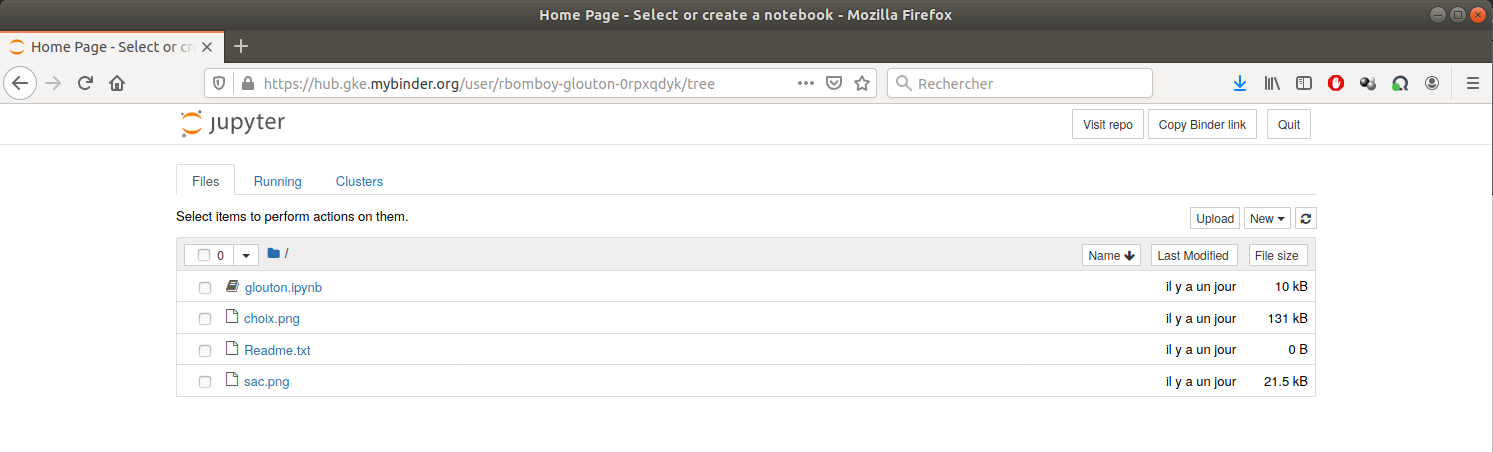
\includegraphics[scale=0.25]{page_sommaire}
\end{center}

Cliquer sur python.ipynb pour éditer le notebook.

\begin{center}
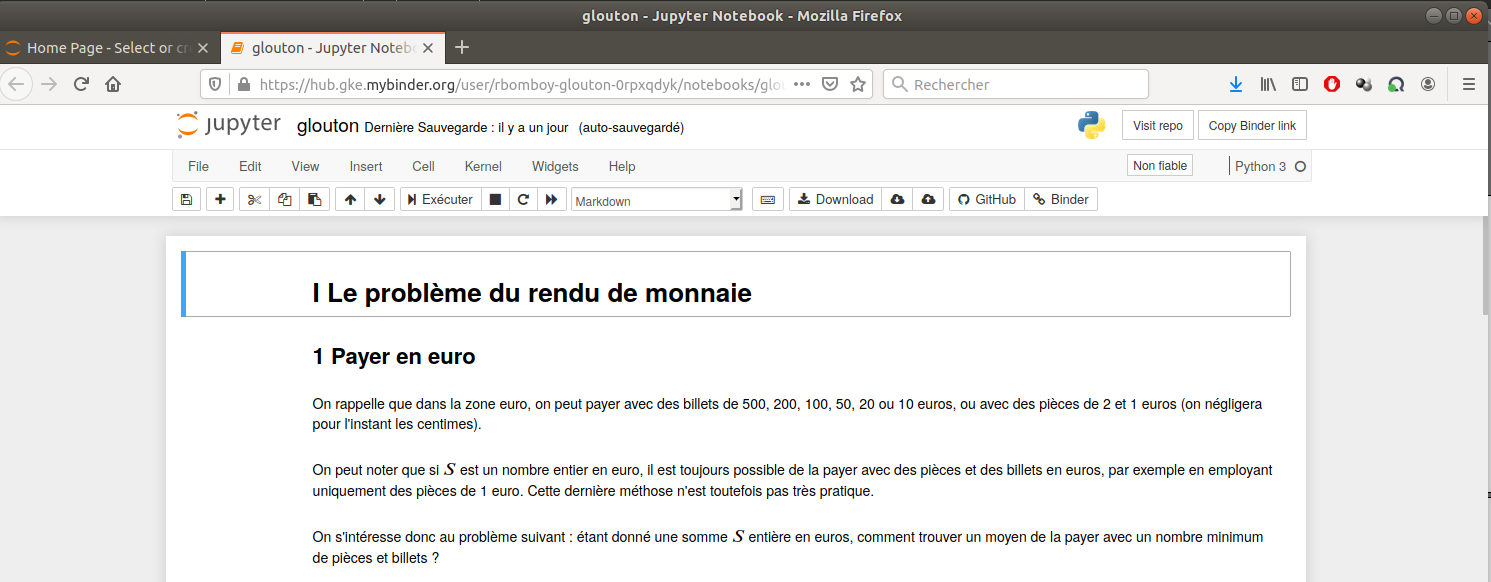
\includegraphics[scale=0.25]{notebook}
\end{center}

On peut alors compléter les cellules contenant du code Python et tester ce code.

\begin{center}
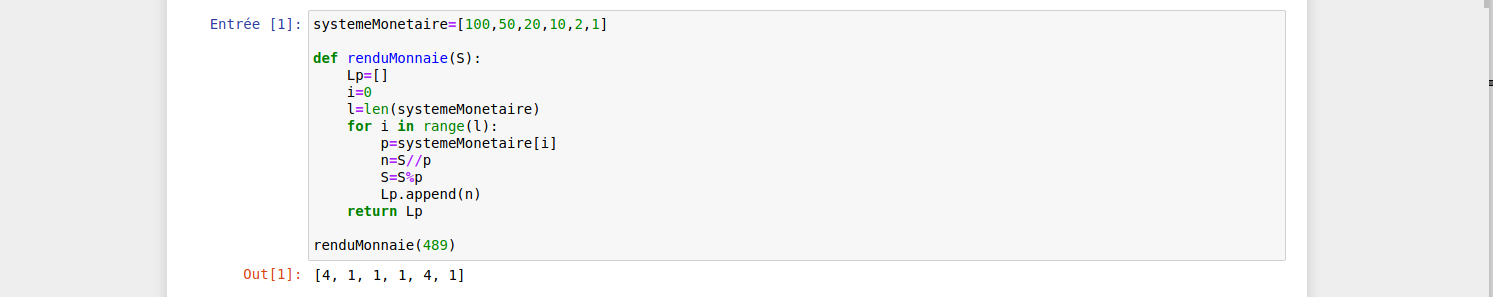
\includegraphics[scale=0.25]{code}
\end{center}
\end{document}